\section{Experiments}

\subsection{Experimental Setup}

\textbf{Dataset and evaluation platform.}
We evaluate ASID on the Eadro-SN dataset, a realistic cloud microservice diagnosis benchmark derived from the Eadro platform~\cite{10172617}. The system comprises 12 microservices with complex inter-service dependencies. Each online inference step consumes a sliding window of preprocessed multimodal tensors: service-level metric features covering CPU, memory, and traffic statistics; log-derived level statistics aggregated per service; and trace edge features over service pairs, including call count and mean duration. \lb{The evaluation protocol uses a fixed case-level train/validation/test split: the training split provides window-level anomaly supervision, the validation split is used only for threshold and temporal-rule selection, and the held-out test split is used only once for final reporting. The 568-step test replay contains 215 anomalous windows and 353 normal windows, corresponding to a positive rate of 37.85\%.}

\lb{For supplementary anomaly-detection generality, we also evaluate ASID on MSDS and RCAEval RE2-TT~\cite{pham2025rcaeval}. MSDS is a microservice anomaly-detection dataset, while RCAEval RE2-TT is a Train Ticket microservice benchmark that supports both window-level anomaly detection and service-level root-cause ranking. The detailed latency, ablation, resource, and overload studies remain on Eadro-SN; MSDS and RE2-TT are used as compact cross-dataset checks.}

\textbf{Online evaluation protocol.}
To faithfully assess online diagnosis capability, we adopt a full-replay online evaluation protocol. The entire test set of 568 time steps is replayed sequentially through the inference engine, where each step triggers one sliding-window inference. All latency measurements are recorded end-to-end, from data loading to diagnosis output, reflecting deployment-oriented online inference rather than isolated batch inference.
\textbf{Evaluation metrics.}
We report the following metrics to jointly assess diagnostic effectiveness and deadline compliance:
\begin{itemize}
    \item \textit{Diagnostic accuracy}: F1 score, precision, recall, and accuracy.
    \item \textit{Deadline compliance}: miss@$D$, the fraction of inference steps exceeding the latency budget $D$.
    \item \textit{\lb{Deadline-effective F1}}: \lb{F1 recomputed after replacing any prediction whose response time exceeds deadline \(D\) with a timely negative output, i.e., \(\tilde{y}(t;D)=\hat{y}(t)\) if \(T(t)\le D\) and \(\tilde{y}(t;D)=0\) otherwise.}
    \item \textit{Tail latency}: p99 and maximum observed latency across all replay steps.
    \item \textit{Resource efficiency}: parameter count, trainable parameter count, GPU peak memory, CPU memory, and host-normalized CPU utilization during online inference.
\end{itemize}

\textbf{Implementation details.}
\lb{ASID uses a frozen truncated GPT-2 backbone with parameter-efficient sparse adaptation.} The service-aware MoE-LoRA adapter uses 4 experts and activates up to two experts per routed representation. The adapter applies rank-4 low-rank updates with moderate service-conditioned routing. The diagnosis decision module aggregates per-service anomaly scores using a guarded top-service temporal strategy. The model is trained for 30 epochs with a batch size of 16 using the AdamW optimizer. \lb{For the Eadro-SN experiments, the prediction-loss weight is 1.0, the MoE load-balancing weight is 0.05, focal-loss parameters are \(\gamma=1.5\) and \(\alpha=0.5\), and additional window or boundary auxiliary losses are disabled. The RCA loss is disabled for Eadro-SN and is enabled only in the separate RCAEval ranking experiment.} Thresholds, adaptive-budget parameters, and temporal decision parameters are selected only on the validation split and then fixed for the held-out test replay. All ASID replay experiments are conducted on a single NVIDIA GeForce RTX 4070 SUPER GPU. \lb{The final serving path uses optimized GPU inference, cached runtime metadata, and low-overhead online postprocessing.}

\subsection{Comparison with Baselines}

We compare ASID against representative baselines from three methodological families.

\textbf{Unsupervised time-series detectors.}
GDN~\cite{deng2021graph}, a graph-based detector applied to log features;
TraceAnomaly~\cite{liu2020unsupervised}, a VAE-based trace anomaly detector;
TranAD~\cite{tuli2022tranad}, a Transformer-based detector applied to log sequences;
Anomaly Transformer~\cite{xu2022anomaly}, an attention-based detector applied to trace features;
and \lb{an MTAD-GAT baseline}~\cite{zhao2020mtadgat} that concatenates all three modalities into a single feature input.
These unsupervised baselines fit normal windows and score deviations at test time.

\lb{\textbf{Multimodal deep baseline.}
We use the public Eadro model~\cite{10172617} under the same data split, retaining the original architecture and reporting its strongest configuration.}

\textbf{Classical supervised methods.}
RBF-SVM~\cite{cortes1995support} and XGBoost~\cite{chen2016xgboost}, both trained and evaluated under the same supervised split as ASID.

\lb{All methods use the same fixed case-level data split. Detection metrics (F1, precision, recall) are computed on the full held-out test set. Latency is measured from end-to-end online replay; all methods use the full 568-step replay sequence, so their tail latencies are directly comparable.}

\begin{table*}[!t]
\caption{\lb{Baseline Comparison on Eadro-SN}}
\label{tab:baseline}
\centering
\renewcommand{\arraystretch}{1.1}
\begin{tabular}{l|ccc|ccc}
\hline
\textbf{Method} & \textbf{F1} & \textbf{Prec.} & \textbf{Rec.} & \textbf{miss@25} & \textbf{p99 (ms)} & \textbf{max (ms)} \\
\hline
\textbf{\lb{ASID (ours)}} & \textbf{0.9838} & \textbf{0.9815} & \textbf{0.9860} & \textbf{0.0\%} & \textbf{16.69} & \textbf{20.04} \\
\hline
\lb{Eadro} & \lb{0.9336} & \lb{0.9189} & \lb{0.9488} & \lb{0.0\%} & \lb{9.64} & \lb{13.67} \\
\lb{XGBoost} & \lb{0.9262} & \lb{0.8922} & \lb{0.9628} & \lb{78.70\%} & \lb{40.15} & \lb{47.71} \\
\lb{RBF-SVM} & 0.8554 & 0.7695 & 0.9628 & 100.0\% & 62.16 & 68.72 \\
GDN & 0.7344 & 0.8343 & 0.6558 & 0.0\% & 20.61 & 24.27 \\
TraceAnomaly & 0.6930 & 0.6556 & 0.7349 & 0.35\% & 22.62 & 27.35 \\
TranAD & 0.6821 & 0.7600 & 0.6186 & 0.0\% & 20.46 & 21.58 \\
Anomaly Trans. & 0.5537 & 0.3835 & 0.9953 & 0.70\% & 24.33 & 28.63 \\
MTAD-GAT & 0.5499 & 0.3792 & 1.0000 & 0.0\% & 20.30 & 21.60 \\
\hline
\end{tabular}
\end{table*}

Table~\ref{tab:baseline} summarizes the results. \lb{Under a 25\,ms tight deadline, several neural time-series detectors satisfy the timing requirement but remain substantially less accurate, with F1 scores between 0.55 and 0.73. Eadro is the strongest external deep baseline, reaching F1\,=\,0.9336 with zero misses at 25\,ms; ASID still improves over it by 5.02 percentage points in F1. Among classical supervised methods, XGBoost reaches F1\,=\,0.9262, but misses 78.70\% of 25\,ms deadlines and remains 5.76 percentage points below ASID in F1. ASID is the only method in the table that combines F1 above 0.98 with zero misses at the 25\,ms operating point.}

\lb{ASID achieves the highest F1 of 0.9838 with 0.0\% deadline misses at 25\,ms, a p99 latency of 16.69\,ms, and a maximum latency of 20.04\,ms under the optimized serving path. The result uses ASID's confidence-adaptive budget.} The confusion matrix is TP\,=\,212, TN\,=\,349, FP\,=\,4, and FN\,=\,3 over the 568-step replay. \lb{Compared with the Eadro model, ASID reduces the remaining detection errors from 29 to 7. Compared with XGBoost, ASID improves F1 by 5.76 percentage points and reduces p99 latency from 40.15\,ms to 16.69\,ms. These results show that adaptive sparse inference improves diagnostic accuracy while meeting a tight 25\,ms online replay deadline.}

\begin{figure*}[!t]
\centering
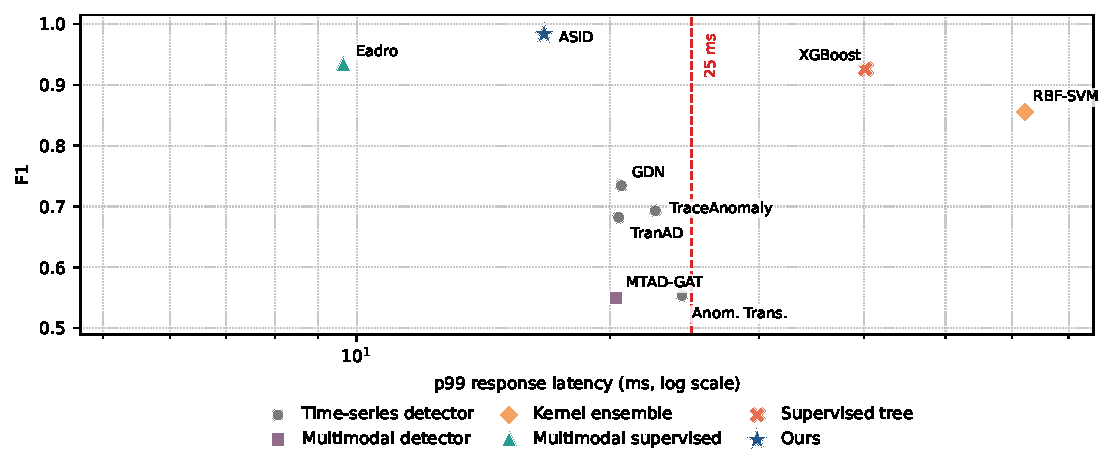
\includegraphics[width=0.92\textwidth]{figures/fig_accuracy_latency_tradeoff.pdf}
\caption{\lb{Accuracy--latency trade-off across external baselines and ASID. ASID reaches the highest F1 while meeting the 25\,ms tight deadline.}}
\label{fig:tradeoff}
\end{figure*}

\subsection{\lb{Cross-Dataset Generality}}

\lb{Eadro-SN is the primary benchmark in this paper. To assess generality beyond a single dataset, Table~\ref{tab:cross_dataset} reports supplementary anomaly-detection results on three datasets: Eadro-SN, MSDS, and RCAEval RE2-TT.}

\begin{table*}[!t]
\caption{\lb{Cross-Dataset Anomaly Detection}}
\label{tab:cross_dataset}
\centering
\renewcommand{\arraystretch}{1.1}
\begin{tabular}{l|l|c|c}
\hline
\textbf{Dataset} & \textbf{Method} & \textbf{F1} & \textbf{p99 (ms)} \\
\hline
\lb{MSDS} & \lb{ASID} & \lb{0.9291} & \lb{29.90} \\
\lb{MSDS} & \lb{TranAD} & \lb{0.8966} & \lb{24.83} \\
\lb{MSDS} & \lb{Anom.\ Trans.} & \lb{0.6250} & \lb{27.64} \\
\lb{RE2-TT} & \lb{ASID} & \lb{0.9180} & \lb{29.96} \\
\lb{RE2-TT} & \lb{ServiceAnomaly} & \lb{0.6420} & \lb{N/R} \\
\lb{RE2-TT} & \lb{DeepTraLog} & \lb{0.4980} & \lb{9.79} \\
\hline
\end{tabular}
\end{table*}

\lb{On MSDS, ASID outperforms TranAD and Anomaly Transformer in F1 under the same supplementary evaluation setting. On RE2-TT, we include the external baselines that we previously ran on the TrainTicket/RCAEval line: ServiceAnomaly as a TrainTicket graph-isomorphism proxy and DeepTraLog as a HetGNN smoke/probe. These two rows are not strict streaming-replay baselines. ASID reaches the best mean F1 of 0.9180 with p99 latency of 29.96\,ms under the replay protocol. The adaptive-budget parameters are selected on each dataset's validation split rather than copied from Eadro-SN. These results show that the sparse multimodal diagnosis design generalizes beyond the primary Eadro-SN benchmark. Eadro-SN remains the only dataset used for the detailed external baseline, ablation, resource, and overload analysis, while RCA-specific RE2-TT baselines are reported separately in Table~\ref{tab:rca}.}

\subsection{Service-Level Root-Cause Ranking}

We further evaluate whether the deviation representation can support service-level root-cause ranking. \lb{This experiment also uses RCAEval RE2-TT, but it is separate from the RE2-TT anomaly-detection row in Table~\ref{tab:cross_dataset}.} It reports the official service-level RCA metrics AC@1, AC@3, AC@5, and Avg@5 on a stratified 30-case test split. We consider two aggregation settings: \emph{early ranking}, which uses only the first three abnormal windows of each case to simulate rapid online diagnosis, and \emph{all-window ranking}, which aggregates over all abnormal windows and is comparable with public RCAEval baselines such as BARO~\cite{pham2024baro} and TraceRCA~\cite{pham2025rcaeval}.

\begin{table*}[!t]
\caption{Service-Level Root-Cause Ranking on RCAEval RE2-TT}
\label{tab:rca}
\centering
\renewcommand{\arraystretch}{1.1}
\begin{tabular}{l|l|cccc}
\hline
\textbf{Method} & \textbf{Aggregation} & \textbf{AC@1} & \textbf{AC@3} & \textbf{AC@5} & \textbf{Avg@5} \\
\hline
\textbf{Root-victim ranking} & early & \textbf{0.9333} & \textbf{1.0000} & \textbf{1.0000} & \textbf{0.9867} \\
Rootness ranking & early & 0.8667 & 1.0000 & 1.0000 & 0.9667 \\
Anomaly-score ranking & early & 0.8333 & 1.0000 & 1.0000 & 0.9533 \\
\hline
Root-victim ranking & all & 1.0000 & 1.0000 & 1.0000 & 1.0000 \\
BARO & all & 0.6667 & 0.8333 & 0.8667 & 0.8067 \\
TraceRCA & all & 0.6333 & 0.7333 & 0.7667 & 0.7267 \\
\hline
\end{tabular}
\end{table*}

\lb{Table~\ref{tab:rca} shows that even directly sorting by anomaly score yields strong early ranking (AC@1\,=\,0.8333). The root-victim ranking branch further improves to AC@1\,=\,0.9333 and Avg@5\,=\,0.9867 under early ranking, and reaches perfect accuracy under all-window ranking. By comparison, BARO and TraceRCA obtain Avg@5 of 0.8067 and 0.7267, respectively. These results confirm that the deviation representation learned for anomaly detection can also support effective service-level root-cause ranking.}

\subsection{Diagnostic Explanation and Routing Case Study}

\lb{Beyond aggregate detection and RCA metrics, we inspect representative online diagnosis outputs to verify that ASID exposes actionable diagnostic evidence. Figure~\ref{fig:case_explanation} shows one abnormal Eadro-SN window whose true root service is \textit{nginx-web-server}; the abnormal services include \textit{compose-post-service}, \textit{home-timeline-service}, \textit{nginx-web-server}, \textit{social-graph-service}, and \textit{user-service}. ASID ranks the true root service first with score 0.7962, followed by \textit{user-service} (0.4180), \textit{compose-post-service} (0.3873), \textit{text-service} (0.3471), and \textit{home-timeline-service} (0.2582). Modality attribution is computed by occluding one modality at a time and measuring the positive drop in the window anomaly score; metrics contribute 85.1\% of the positive evidence, logs contribute 14.9\%, and traces contribute 0.0\% for this window. The current top-service window score is 0.5338, and the alert state is retained as temporal evidence for the online decision. For \textit{nginx-web-server}, the adaptive budget selects \(k(t)=2\), so both experts are used for this uncertain window; the selected route assigns 68.0\% weight to expert 3 and 32.0\% to expert 0. Across all services in the window, top-1 expert shares are 25.0\%, 16.7\%, 25.0\%, and 33.3\%, with normalized router entropy 0.464.}

\lb{This case study illustrates how the same online inference pass yields four complementary signals: service-level anomaly ranking, modality-level evidence, temporal window evidence, and sparse routing diagnostics. We use these signals for diagnostic interpretation; the quantitative RCA claims remain confined to the RCAEval evaluation in Table~\ref{tab:rca}.}

\begin{figure*}[!t]
\centering
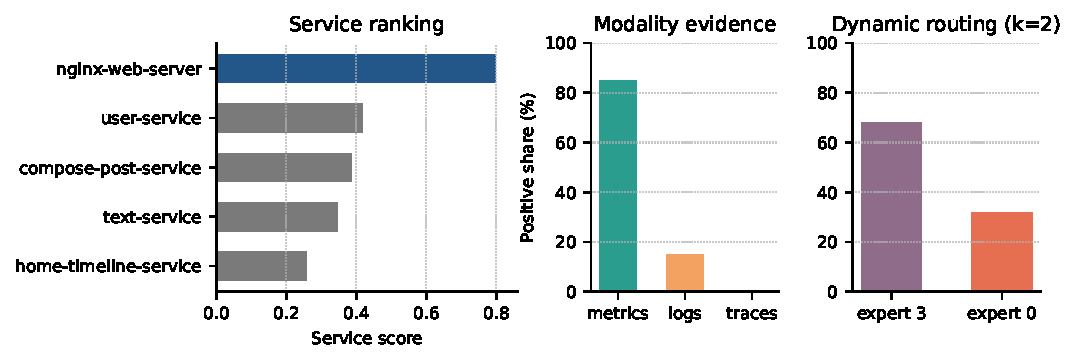
\includegraphics[width=0.92\textwidth]{figures/fig_case_explanation.pdf}
\caption{\lb{Visualization of the representative diagnostic explanation. The true root service is ranked first, metrics dominate the positive modality evidence, and the adaptive budget selects \(k(t)=2\) for the root-service route in this uncertain window.}}
\label{fig:case_explanation}
\end{figure*}

\subsection{Ablation Study}

We conduct comprehensive ablation experiments to verify the contribution of each design component. All ablation variants use the same data split and validation-only threshold selection, and are evaluated under online replay. \lb{Detection metrics are the primary ablation evidence; latency columns report the measured replay path for each variant, while Table~\ref{tab:baseline} reports the optimized serving latency of the final model.}

\textbf{Temporal backbone ablation.}
\lb{To examine whether the GPT-2 backbone can be replaced by conventional compact sequence models, we keep the same multimodal encoders, fusion projection, prediction-deviation representation, and diagnosis heads, and replace only the temporal backbone with a GRU, a causal Transformer, or a temporal convolutional network (TCN). These alternatives substantially underperform in diagnostic accuracy: the GRU reaches F1\,=\,0.9017, the causal Transformer reaches F1\,=\,0.9119, and the strongest alternative, TCN, reaches F1\,=\,0.9306. Their accuracy remains 5.32--8.21 percentage points below ASID, indicating that the frozen truncated GPT-2 backbone with parameter-efficient sparse adaptation provides useful temporal representation capacity beyond simply using a compact sequence model.}

\textbf{Architecture ablation.}
We evaluate the effect of the service-aware MoE-LoRA adapter by comparing the full model against two degraded variants: (i)~\textit{single shared adapter}, which replaces the mixture-of-experts adapter with one shared low-rank adapter, and (ii)~\textit{without service-conditioned routing}, which removes the service prior from the MoE adapter. As shown in Table~\ref{tab:ablation}, removing MoE causes F1 to drop from 0.9838 to 0.9152 while maintaining low latency, confirming that sparse expert specialization is critical for diagnostic accuracy. \lb{Removing the service-conditioned prior preserves most accuracy (F1\,=\,0.9721) but degrades tail latency to p99\,=\,83.70\,ms, indicating that service-conditioned routing stabilizes inference timing.}
\textbf{Modality ablation.}
To validate the multimodal fusion design, we compare the full three-modality model against all possible dual-modality and conceptually reduced configurations. Full modality achieves the best F1 of 0.9838. \lb{Removing logs (metrics+traces) reduces F1 to 0.9192. Removing traces (metrics+logs, F1\,=\,0.7909) or metrics (logs+traces, F1\,=\,0.7951) leads to more significant degradation.} These results confirm that all three modalities provide complementary information for the deviation representation, and that the unified encoding design is essential.

\textbf{Decision strategy ablation.}
We ablate the diagnosis decision module by comparing four strategies: no temporal filtering, temporal confirmation only, confirmation with high-confidence bypass, and the full guarded temporal decision. \lb{The full strategy achieves the best F1 and the lowest tail latency, while removing temporal logic causes F1 to drop to 0.9298 and increases tail latency.} This validates that the bounded alert state machine contributes to both accuracy and timing stability.

\textbf{Adapter capacity ablation.}
We vary the LoRA rank to assess whether performance gains are attributable to increased parameter count. As shown in Table~\ref{tab:ablation}, rank-2 (smaller) achieves F1\,=\,0.9721 with p99\,=\,82.17\,ms, and rank-8 (larger) yields F1\,=\,0.9354 with p99\,=\,71.97\,ms. \lb{Neither outperforms the default rank-4 configuration. We therefore avoid interpreting larger rank as a monotonic capacity improvement; on this data split, larger adapters may overfit the validation set.}

\textbf{\lb{Sparse-budget ablation.}}
\lb{We further isolate the effect of the confidence-adaptive budget in Table~\ref{tab:budget_ablation}. A fixed one-expert budget reduces F1 to 0.9676, showing that always using the cheapest route weakens expert specialization. A fixed two-expert budget reaches the same F1 as the final model but evaluates two experts for every window. The confidence-adaptive policy preserves F1\,=\,0.9838 while reducing mean expert evaluations, avoiding unnecessary expert computation on confident windows while preserving the full two-expert route for uncertain contexts. The latency values in this table come from controlled budget-ablation runs and are intended only for within-table comparison; the optimized serving path in Table~\ref{tab:baseline} reports the deployment latency of the final model.}

\begin{table*}[!t]
\caption{Ablation Study Results}
\label{tab:ablation}
\centering
\renewcommand{\arraystretch}{1.1}
\begin{tabular}{l|cccc|cc}
\hline
\textbf{Configuration} & \textbf{F1} & \textbf{P} & \textbf{R} & \textbf{Acc} & \textbf{p99} & \textbf{max} \\
 & & & & & \textbf{(ms)} & \textbf{(ms)} \\
\hline
\textbf{ASID (full)} & \textbf{0.9838} & \textbf{0.9815} & \textbf{0.9860} & \textbf{0.9877} & \textbf{16.69} & \textbf{20.04} \\
\hline
\multicolumn{7}{l}{\textit{Temporal backbone}} \\
\hline
GRU & 0.9017 & 0.8340 & 0.9814 & 0.9190 & 32.75 & 42.49 \\
causal Transformer & 0.9119 & 0.8661 & 0.9628 & 0.9296 & 29.88 & 39.61 \\
TCN & 0.9306 & 0.8966 & 0.9674 & 0.9454 & 50.60 & 66.53 \\
\hline
\multicolumn{7}{l}{\textit{Architecture}} \\
\hline
single shared adapter & 0.9152 & 0.8798 & 0.9535 & 0.9331 & 58.02 & 75.66 \\
no service routing & 0.9721 & 0.9721 & 0.9721 & 0.9789 & 83.70 & 166.75 \\
\hline
\multicolumn{7}{l}{\textit{Modality}} \\
\hline
metrics+traces & 0.9192 & 0.9128 & 0.9256 & 0.9384 & 73.74 & 112.32 \\
metrics+logs & 0.7909 & 0.8626 & 0.7302 & 0.8539 & 69.89 & 88.34 \\
logs+traces & 0.7951 & 0.8359 & 0.7581 & 0.8521 & 56.55 & 113.63 \\
\hline
\multicolumn{7}{l}{\textit{Decision strategy}} \\
\hline
no temporal & 0.9298 & 0.8797 & 0.9860 & 0.9437 & 77.99 & 142.53 \\
confirm only & 0.9417 & 0.9091 & 0.9767 & 0.9542 & 85.47 & 110.09 \\
confirm+high bypass & 0.9745 & 0.9722 & 0.9767 & 0.9806 & 94.43 & 159.01 \\
\hline
\multicolumn{7}{l}{\textit{Adapter capacity}} \\
\hline
rank-2 & 0.9721 & 0.9721 & 0.9721 & 0.9789 & 82.17 & 103.07 \\
rank-4 (default) & 0.9838 & 0.9815 & 0.9860 & 0.9877 & 16.69 & 20.04 \\
rank-8 & 0.9354 & 0.8974 & 0.9767 & 0.9489 & 71.97 & 104.17 \\
\hline
\end{tabular}
\end{table*}

\begin{table}[!t]
\caption{\lb{Sparse-Budget Policy Ablation}}
\label{tab:budget_ablation}
\centering
\footnotesize
\renewcommand{\arraystretch}{1.1}
\begin{tabular}{l|cccc}
\hline
\textbf{Budget policy} & \textbf{F1} & \textbf{mean experts} & \textbf{p99} & \textbf{max} \\
 & & & \textbf{(ms)} & \textbf{(ms)} \\
\hline
\lb{fixed one expert} & \lb{0.9676} & \lb{1.000} & \lb{75.71} & \lb{92.91} \\
\lb{fixed two experts} & \lb{0.9838} & \lb{2.000} & \lb{74.04} & \lb{84.87} \\
\textbf{\lb{confidence-adaptive}} & \textbf{\lb{0.9838}} & \textbf{\lb{1.890}} & \textbf{\lb{68.42}} & \textbf{\lb{91.19}} \\
\hline
\end{tabular}
\end{table}

\textbf{Service prior strength operating region.}
\lb{We further analyze the sensitivity to the service-conditioned routing prior strength $\lambda$ in Table~\ref{tab:prior}. Moderate values ($\lambda{=}0.5$ and $\lambda{=}0.6$) achieve the best F1 of 0.9838. A weaker prior ($\lambda{=}0.4$) yields F1\,=\,0.9354, while an overly strong prior ($\lambda{=}0.75$) reduces F1 to 0.9745. These results show that a moderate service prior stabilizes diagnostic performance.}

\begin{table*}[!t]
\caption{\lb{Sensitivity to Service Prior Strength $\lambda$}}
\label{tab:prior}
\centering
\renewcommand{\arraystretch}{1.1}
\begin{tabular}{c|cccc}
\hline
$\lambda$ & \textbf{F1} & \textbf{P} & \textbf{R} & \textbf{Acc} \\
\hline
0 (no prior) & 0.9721 & 0.9721 & 0.9721 & 0.9789 \\
0.4 & 0.9354 & 0.8974 & 0.9767 & 0.9489 \\
0.5 & \textbf{0.9838} & \textbf{0.9815} & \textbf{0.9860} & \textbf{0.9877} \\
\textbf{0.6} & \textbf{0.9838} & \textbf{0.9815} & \textbf{0.9860} & \textbf{0.9877} \\
0.75 & 0.9745 & 0.9722 & 0.9767 & 0.9806 \\
\hline
\end{tabular}
\end{table*}

\subsection{Real-Time System Evaluation}

To validate that ASID operates as an online diagnosis system rather than an offline detector evaluated post-hoc, we present three groups of evidence: multi-deadline analysis, overload stress testing, and resource efficiency.

\textbf{Multi-deadline analysis.}
\lb{Figure~\ref{fig:deadline_tradeoff} reports the diagnostic performance of ASID under varying latency budgets $D$. We use 25\,ms as a tight operating point because it is close to the optimized serving tail while remaining practical for online diagnosis. At 25\,ms, ASID achieves 0.0\% miss rate and preserves F1\,=\,0.9838. Tightening the budget to 20\,ms remains near the observed tail, while 15\,ms causes a 4.40\% miss rate and a deadline-effective F1 of 0.9645. A 10\,ms budget is below this serving path's stable operating region. These results show where ASID remains timely and where latency pressure begins to affect diagnosis quality.}

\begin{figure}[!t]
\centering
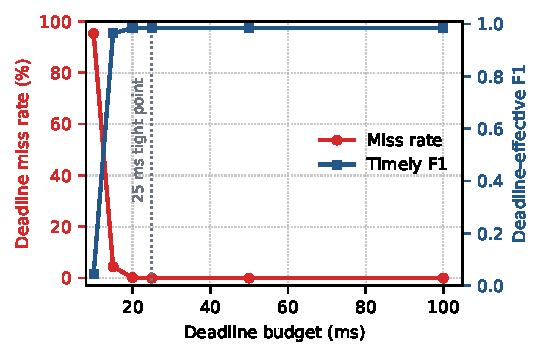
\includegraphics[width=\linewidth]{figures/fig_deadline_tradeoff.pdf}
\caption{\lb{Multi-deadline operating curve. The optimized serving path keeps all windows below 25\,ms; degradation appears only when the deadline is tightened below the observed tail.}}
\label{fig:deadline_tradeoff}
\end{figure}

\begin{figure}[!t]
\centering
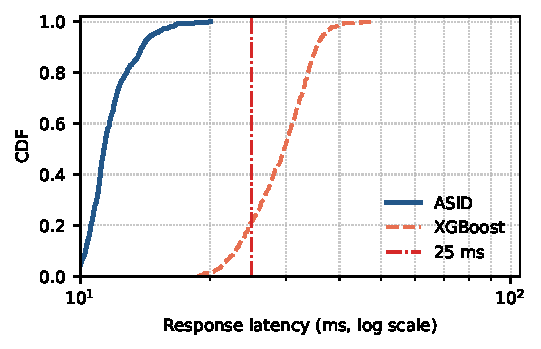
\includegraphics[width=\linewidth]{figures/fig_latency_cdf.pdf}
\caption{\lb{Online replay latency CDF. ASID remains below the 25\,ms tight operating point, while XGBoost has a heavier tail and substantially lower diagnostic F1.}}
\label{fig:latency_cdf}
\end{figure}

\textbf{Trace-driven overload analysis.}
\lb{We analyze workload overload by replaying inference requests at varying arrival intervals in a single-server queue model driven by the actual per-step processing times from the final confidence-adaptive serving replay. Table~\ref{tab:overload} reports deadline misses under the 25\,ms tight operating point. ASID sustains 0.0\% miss rate up to 6.7$\times$ the nominal load and remains near the measured serving tail through 8$\times$ load, where the miss rate is 1.06\%. At 10$\times$ load, the system saturates and queueing delay dominates the response time.}

\begin{table*}[!t]
\caption{\lb{Trace-Driven Overload Analysis for ASID}}
\label{tab:overload}
\centering
\renewcommand{\arraystretch}{1.1}
\begin{tabular}{cc|ccc}
\hline
\textbf{Interval} & \textbf{Load} & \textbf{miss@25} & \textbf{thpt} & \textbf{response} \\
\textbf{(ms)} & & & \textbf{(win/s)} & \textbf{p99 (ms)} \\
\hline
200 & 0.5$\times$ & 0.00\% & 5.01 & 16.69 \\
\textbf{100} & \textbf{1.0$\times$} & \textbf{0.00\%} & \textbf{10.02} & \textbf{16.69} \\
50 & 2.0$\times$ & 0.00\% & 20.03 & 16.69 \\
25 & 4.0$\times$ & 0.00\% & 40.04 & 16.69 \\
\lb{20} & \lb{5.0$\times$} & \lb{0.00\%} & \lb{50.04} & \lb{16.69} \\
\lb{15} & \lb{6.7$\times$} & \lb{0.00\%} & \lb{66.70} & \lb{17.87} \\
\lb{12.5} & \lb{8.0$\times$} & \lb{1.06\%} & \lb{80.02} & \lb{24.45} \\
10 & 10.0$\times$ & 97.89\% & 84.99 & 1008.42 \\
\hline
\end{tabular}
\end{table*}

\textbf{Resource efficiency.}
\lb{Table~\ref{tab:resource} compares the resource and runtime footprint of ASID with the two strongest full-replay baselines. ASID contains 61.91M neural parameters, but only 2.06M (3.33\%) are trainable because the GPT-2 backbone is frozen; the trainable MoE adapter accounts for 0.90M parameters. Under the optimized serving path, the CUDA peak allocation is 149.43\,MB. The Eadro model is compact and faster than ASID but less accurate. XGBoost has no neural parameters; we report the serialized model footprint. At the 25\,ms tight operating point, ASID and Eadro have zero misses, while XGBoost has a heavier tail. CPU utilization is normalized by the 16 logical cores on the evaluation host.}

\begin{table*}[!t]
\caption{\lb{Resource and Runtime Footprint During Full Online Replay}}
\label{tab:resource}
\centering
\renewcommand{\arraystretch}{1.1}
\begin{tabular}{p{0.16\textwidth}|c|p{0.14\textwidth}|p{0.15\textwidth}|ccc|cc}
\hline
\textbf{Method} & \textbf{F1} & \textbf{Neural params} & \textbf{Model} & \textbf{GPU} & \textbf{CPU RSS} & \textbf{CPU util.} & \textbf{p99} & \textbf{miss@25} \\
 & & \textbf{total / trainable (M)} & \textbf{footprint} & \textbf{peak (MB)} & \textbf{p99 (MB)} & \textbf{host p95} & \textbf{(ms)} & \\
\hline
\textbf{\lb{ASID (ours)}} & \textbf{0.9838} & \textbf{\lb{61.91 / 2.06}} & \textbf{0.90M MoE adapter} & \textbf{149.43} & \textbf{1256.34} & \textbf{6.51\%} & \textbf{16.69} & \textbf{0.0\%} \\
\lb{Eadro} & \lb{0.9336} & \lb{0.144 / 0.144} & \lb{CPU model} & \lb{--} & \lb{218.25} & \lb{--} & \lb{9.64} & \lb{0.0\%} \\
\lb{XGBoost} & \lb{0.9262} & \lb{N/A} & \lb{32.65\,MB} & \lb{--} & \lb{--} & \lb{--} & \lb{40.15} & \lb{78.70\%} \\
\hline
\end{tabular}
\end{table*}

\lb{Across ASID ablations, GPU peak memory remains consistently around 260\,MB (258.90--261.53\,MB), and the optimized serving path further reduces the final replay peak to 149.43\,MB. These results place ASID at the highest-F1 operating point among the evaluated methods that meet the 25\,ms tight deadline with zero misses.}
